\documentclass{article}
\usepackage[utf8]{inputenc}

\usepackage{amsfonts}
\usepackage{amssymb}
\usepackage{amsmath}
\usepackage{amsthm}
\usepackage{enumitem}

\usepackage{bbold}
\usepackage{bm}
\usepackage{graphicx}
\usepackage{color}
\usepackage{hyperref}
\usepackage[margin=2.5cm]{geometry}

\begin{document}

% ==============================================================================

\title{\Large{INFO8006: Project 3 - Report}}
\vspace{1cm}
\author{\small{\bf Louis HOGGE - s192814} \\ \small{\bf Emilien LECLERC - s190701}}

\maketitle

% ==============================================================================

\section{Bayes filter}

\begin{enumerate}[label=\alph*.,leftmargin=*]
    \item Le "sensor model" du "rusty sensor" calcule la distance approximative entre le ghost et pacman en additionnant leur Manhattan distance et un "noise". Celui-ci est trouvé en faisant la différence entre une variable aléatoire Binomiale et la moyenne. La variable aléatoire Binomiale correspond au nombre de succès de n essais i.i.d. de Bernoulli et la moyenne se calcule en multipliant le nombre d'essaies par la probabilité de réussite.
    \item Un exemple de "unified parametrized transition model" duquel les ghosts "scared", "afraid" et "confused" peuvent être dérivés est le suivant: Avec comme unique paramètre l'état actuel du jeux (qui comprend la position de pacman, le type et la position du ghost et la position des murs), le modèle commence par identifier les déplacements possibles du ghost. Ensuite, si le ghost est de type "confused", un coefficient de $1$ est associé à chaque mouvement légal. Si ce n'est pas le cas, la distance actuelle entre le ghost et pacman est calculée via la technique de la Manhattan distance. Après cela, le modèle détermine les distances entre chacune des futurs positions du ghost (déterminées plus haut) et celle de pacman en utilisant la même technique. Si la nouvelle distance est plus grande ou égale à celle actuelle alors, suivant le type du ghost, un coefficient est donné au mouvement qui permet d'accéder à la futur position (si le ghost est de type "afraid" ce coefficient vaut $2$, s'il est de type "scared" il vaut $2^{3}$). Sinon, dans le cas où elle est plus petite, un coefficient $1$ est attribué. On termine par normaliser les coefficients associés aux différents mouvements en les divisant par leur somme.
\end{enumerate}

\section{Implementation}

\begin{enumerate}[label=\alph*.,leftmargin=*]
    \item \textbf{\textit{Leave empty.}}
\end{enumerate}

\section{Experiment}

\begin{enumerate}[label=\alph*.,leftmargin=*]
    \item L'incertitude du "belief state" peut être mesurée en observant la proximité ou non entre les positions fournies par le "belief state" et la position moyenne du ghost, proportionnellement à leurs probabilités.
    \item La qualité du "belief state" peut être mesurée en observant la proximité ou non entre les positions fournies par le "belief state" et la véritable position de pacman, proportionnellement à leurs probabilités.
    \item \newpage
    \begin{figure}[h!]
        \centering
        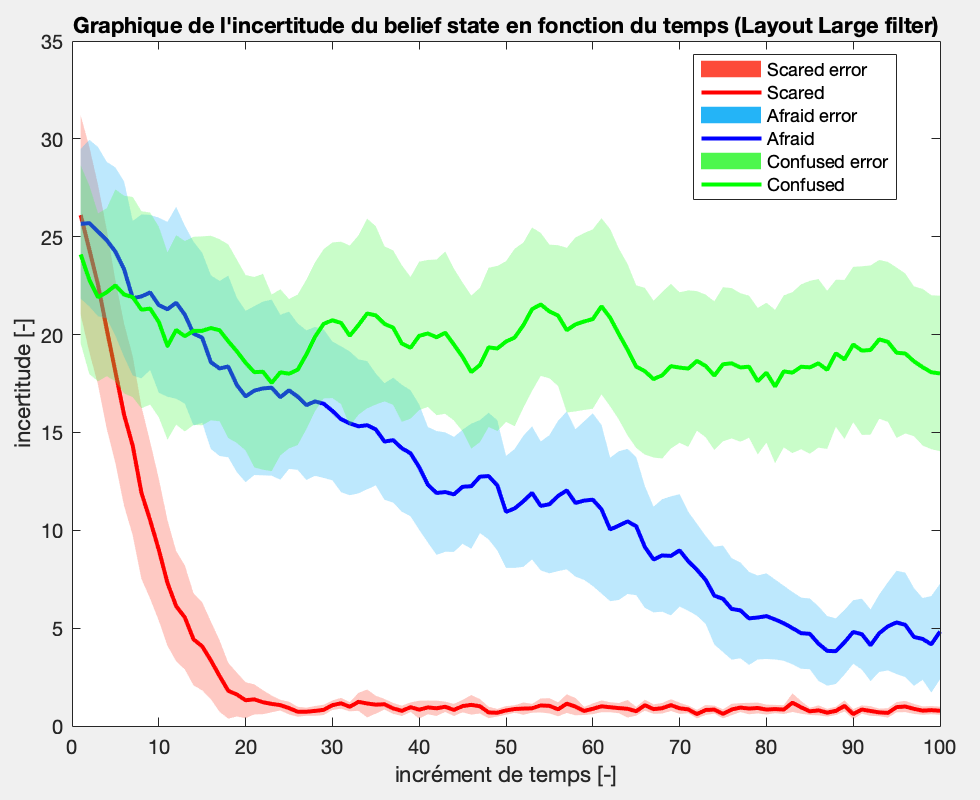
\includegraphics[scale=0.75]{i.png}
    \end{figure}
    \begin{figure}[h!]
        \centering
        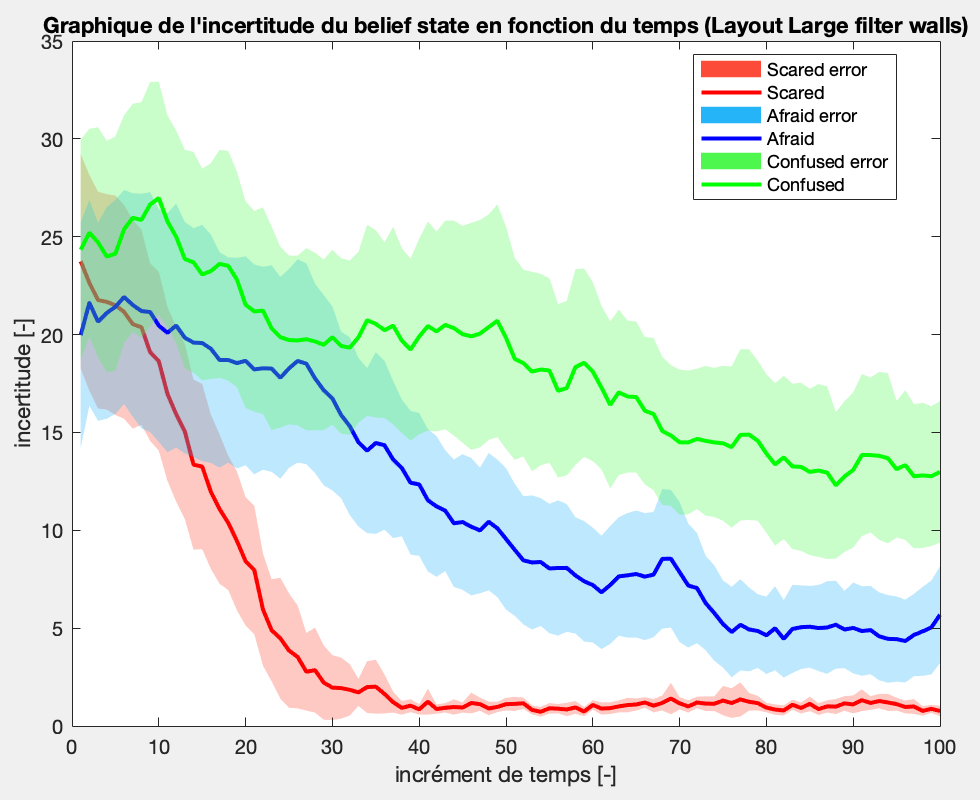
\includegraphics[scale=0.75]{iw.png}
    \end{figure}
    \newpage
    \begin{figure}[h!]
        \centering
        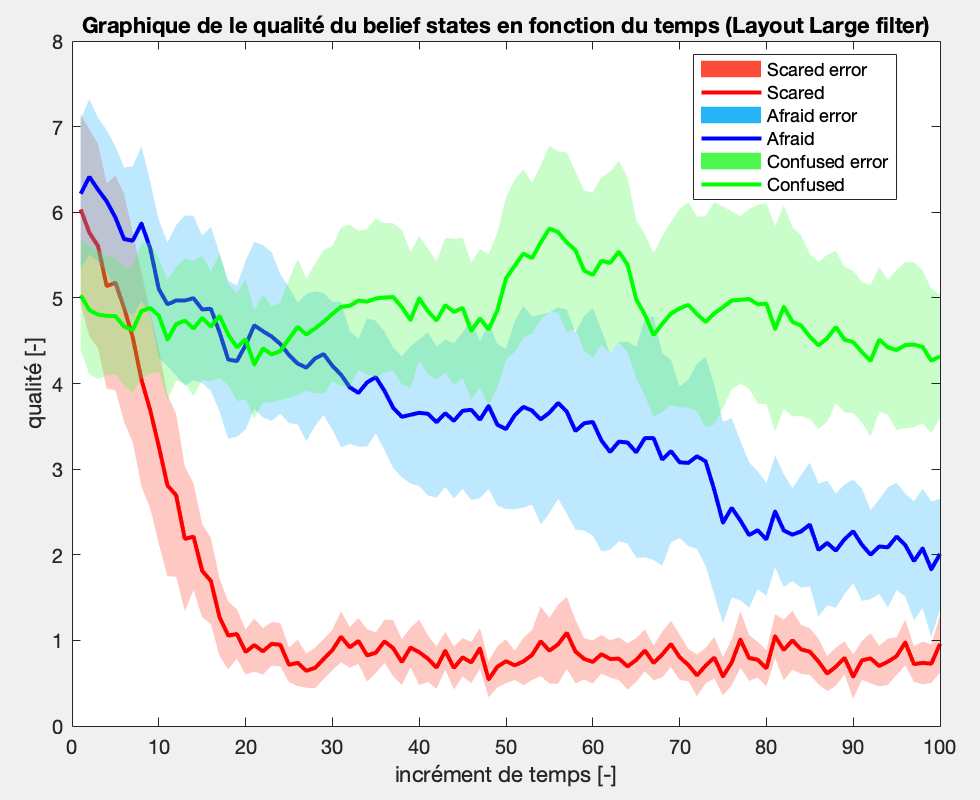
\includegraphics[scale=0.75]{q.png}
    \end{figure}
    \begin{figure}[h!]
        \centering
        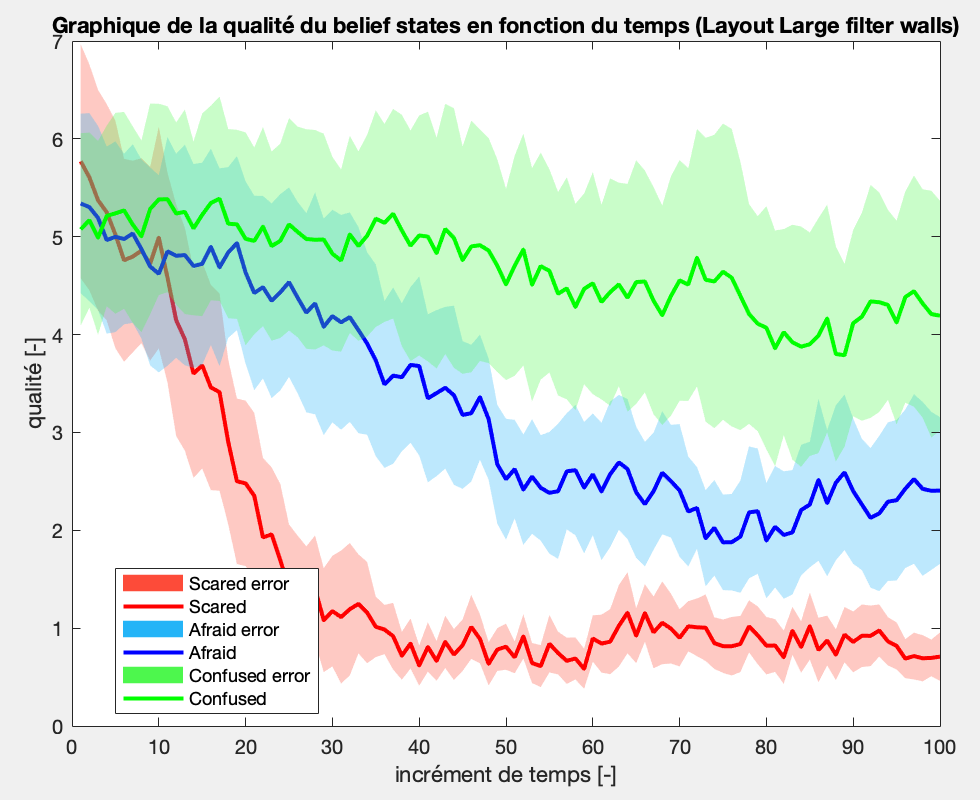
\includegraphics[scale=0.75]{qw.png}
    \end{figure}
    \newpage
    \item  Dans le "transition model", on sait que les ghosts de types "scared" et "afraid" ont une plus grande probabilité de choisir un mouvement qui les éloigne de pacman, d'où l'importance de connaître sa position. La probabilité de sortie du "transition model" est donc impactée et vient à son tour influencer (dans le "get update belief") la contribution des anciens "belief state" dans la création du nouveau. On peut d'ailleurs remarquer sur les graphiques que les mesures des ghosts de types "afraid" et "scared", prenant en compte la position de pacman, convergent alors que celles du ghost de type "confused", qui ne s'intéresse pas à la position de pacman, ne convergent pas.
    \item Dans le "sensor model" le nombre d'essaies de la binomiale (qui en est la sortie) est calculé en fonction de la "sensor variance". Cette sortie influe ensuite sur les probabilités placées dans le "belief state" (qui est la sortie du "get updated belief") en les pondérant.
    \item Une première possibilité serait de trouver la position relative à la probabilité la plus grande du "belief state". Ensuite, en connaissant la liste actuelle d'actions légales de pacman, il suffirait de choisir le mouvement rapprochant pacman de la position déterminée plus haut.
    \\
    \\
    Une deuxième possibilité serait de déterminer un nuage de positions correspondant à une concentration de grandes probabilités dans le "belief state". Après cela, en connaissant la liste actuelle d'actions légales de pacman, il suffirait de choisir le mouvement permetant à pacman de naviguer dans le lieu déterminé plus haut.
    \item \textbf{\textit{Leave empty.}}
\end{enumerate}

% ==============================================================================

\end{document}
